\chapter{Introduction}
\label{c:introduction}
\newcounter{foot}
\setcounter{foot}{1}
Inquiring about the origins of a phenomenon, 
as opposed to merely describing its present state, often 
leads to profound new discoveries. Biology provides a 
wealth of examples. 
Darwin asked the question of the origins of species diversity and 
thus discovered evolution by natural selection. Pasteur
wondered about the origins of life and thus
discovered the role of bacteria in 
human diseases. My approach in this book is going to 
be similar. In order to advance our understanding 
of human language and cognition, I propose to address
the fundamental question how language 
and meaning might ever have originated. I will not do 
this by a historical reconstruction, nor by an 
empirical investigation of child language acquisition or 
by examining data from the birth of new
languages.\footnote{
There has been a renewed interest the last five
years in the 
question of the origins of language from these various 
perspectives. \cite{Hurford:1998} contains 
a representative sample of the most recent work. 
Other samples of recent research 
can be found in \cite{Hawkins:1992} and \cite{Velichkovsky:1996}. 
}
Rather, 
I will pose the question in a completely general way: 
how can a physically embodied autonomous agent \is{agent} arrive 
at a repertoire of categories for conceptualising his
world and how can a group of such agents ever develop 
a shared communication system with the same complexity 
as human natural languages? 

\section{The Talking Heads experiment}

For centuries, philosophers, linguists, psychologists and 
neuroscientists have been groping with the amazing capacities
of the mind. By necessity, they have been doing this through
thought experiments or by observing human behaviour and
brain anatomy. Although this has generated a wealth
of insights,\footnote{Attempts are made to bring together the insights from various
disciplines to establish a true ``cognitive science''. 
\cite{Osherton:1995} contains an introduction into some of the main 
research trends in this very diverse scientific field. 
See also \cite{Luger:1994}. The work reported in the present book can be 
classified as theoretical
cognitive science because I try to formulate and test
the operational adequacy of possible models for the 
origins of language and meaning but do not claim nor
give any evidence that these models are also valid for
human cognition, just as the study of aerodynamics and 
aircraft design may help to understand how birds can 
fly but is more generic than its biological 
implementations.}
everyone involved in this research must surely 
agree that we are still lacking adequate models, 
particularly for higher order cognitive functions like language
processing, and definitely for understanding how such 
functions may have arisen. 
To discover or test such models, it therefore
remains useful to do experiments with artificial systems.
We can build robots that receive sensory inputs
through a camera or other sensors, give them computational 
power and memory, and empower them 
for action in the world by adding actuators. Given such a 
set-up, we can precisely examine the operational adequacy 
of an hypothesis. For example, if someone proposes
a process for segmenting images, we can test this process 
by capturing streams of images through a camera and 
see whether the process is indeed capable of performing 
segmentation. When someone proposes a process 
for parsing sentences, we 
can implement this process and confront it with a series of 
example sentences to measure success and failure. 
How else can we test the operational adequacy of a proposed
cognitive model, given the enormous complexity involved? 
Of course, building an artificial system in no way proves
that the principles that were used to construct it are valid
for natural systems. But it is an enormously valuable 
source of insight for approaching the extraordinarily 
complex phenomena observed in human cognition. 


\begin{figure}[htbp]
  \centerline{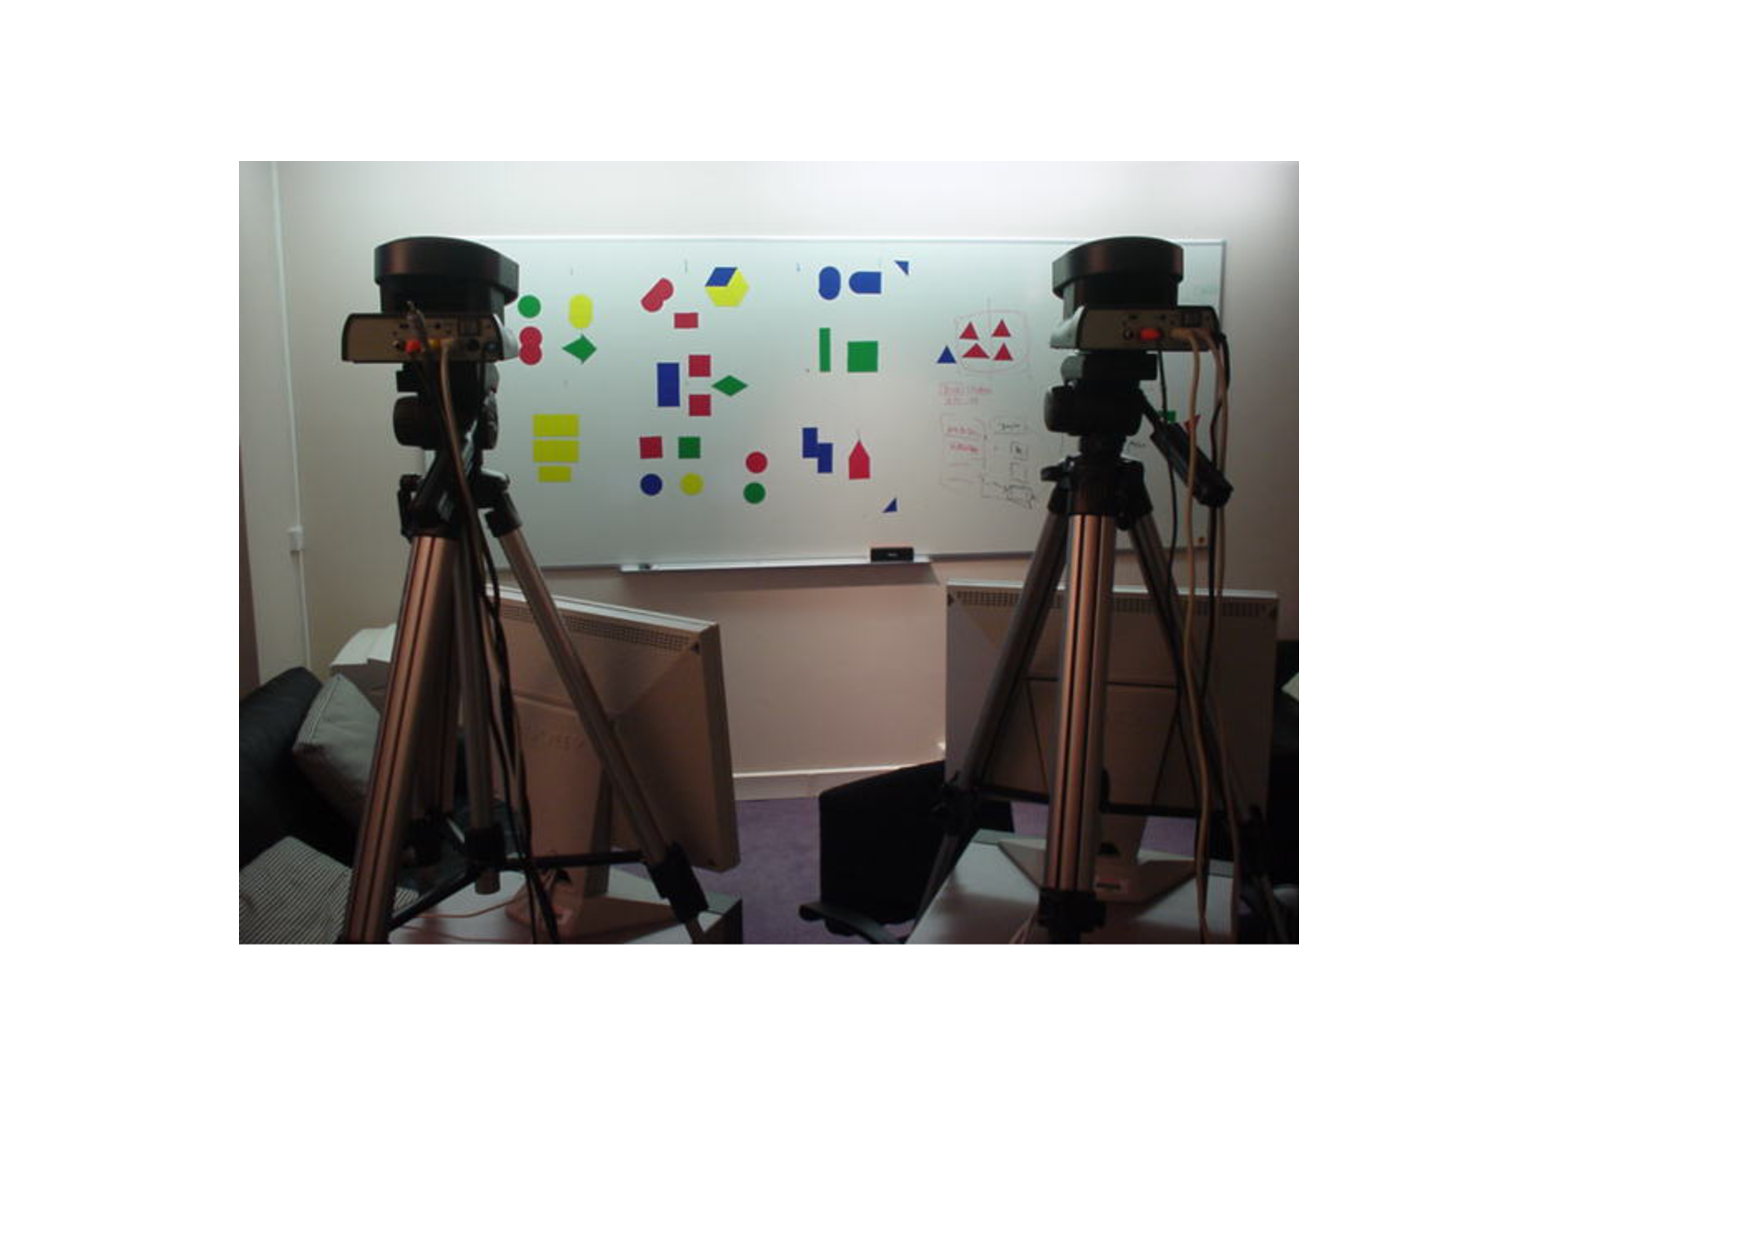
\includegraphics[width=.65\textwidth]{./chap1/figs/heads.pdf}}
\caption{Two Talking Heads are shown {\bfshape a1} and 
{\bfshape a2} each seeing the scene on the white board from a slightly different viewpoint.}
\label{f:plate1}
\end{figure}

The Talking Heads experiment follows this research strategy. \is{Talking Heads Experiment}
It features an enormously challenging experimental
infrastructure to explore how a cognitive
system, like the one underlying human language, might
be able to bootstrap itself into interaction 
with other cognitive systems and driven by increasing
challenges from the environment. The experiment
involves a set of robotic ``Talking Heads'' engaged in language
games, with each other or with human interlocutors, 
about real world scenes they perceive through their sensors
(see Figures \ref{f:plate1} and \ref{f:plate2}).
The robots use vision as major sensory source. They are located in
different places in the world and connected through the Internet. 
Two robotic agents can only engage in an interaction when they 
are instantiated in robot bodies in a shared physical environment. 
After an exchange, an agent can teleport himself to another body in 
another location and engage in interactions there. 


\begin{figure}[htbp]
  \centerline{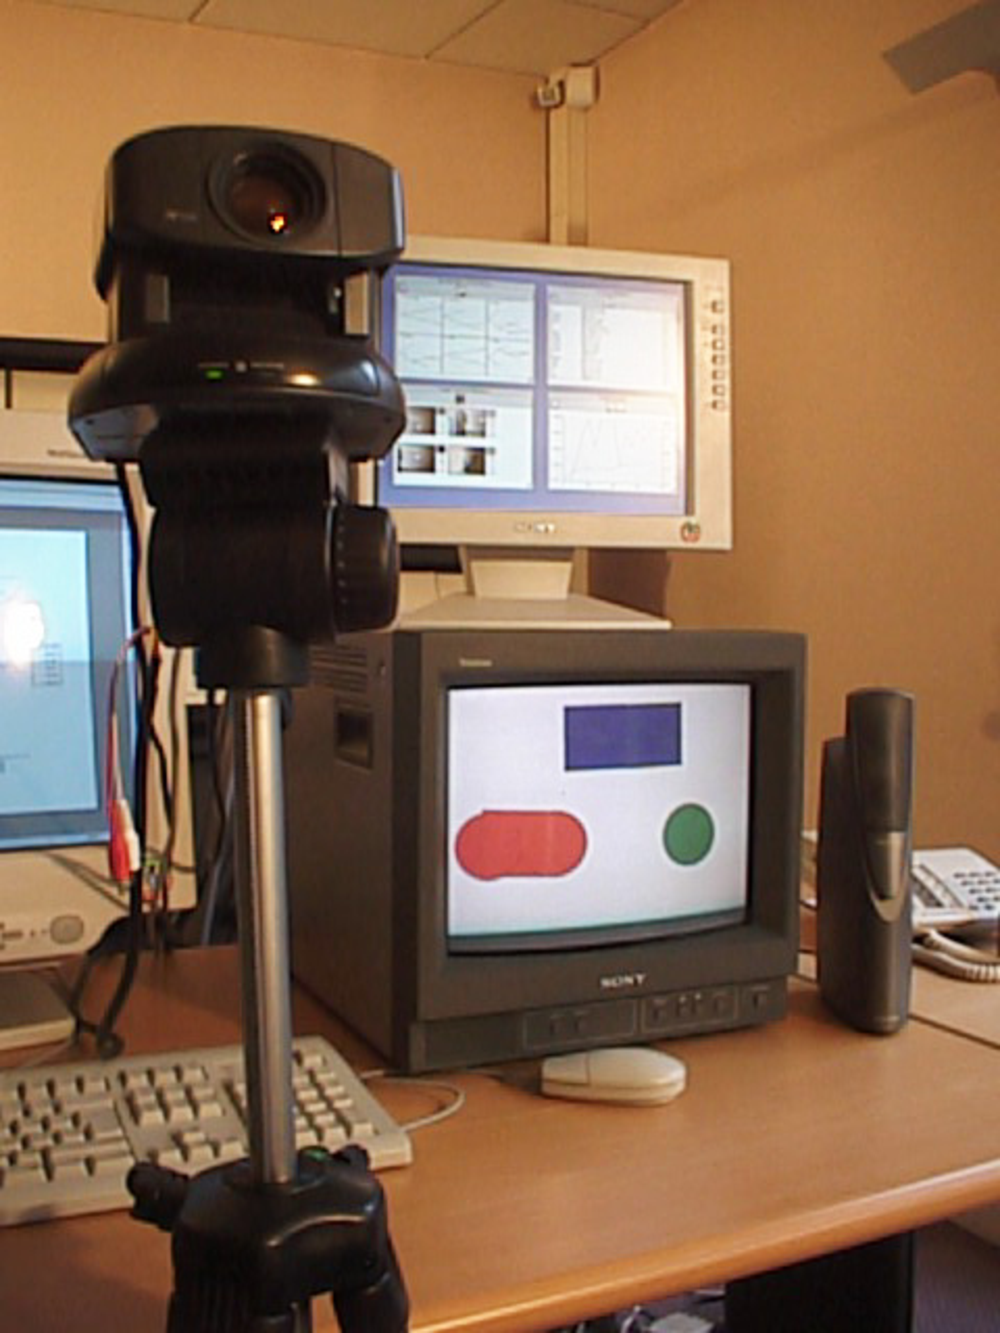
\includegraphics[width=.40\textwidth]{./chap1/figs/head.pdf}}
\caption{A single ``Talking Head''. There is a camera oriented towards a
white board. The bottom screen shows what the camera observes. The top right screen shows the result of processing.
A loudspeaker reproduces the utterances of the agent. }
\label{f:plate2}
\end{figure}

The agents' categorisations of
the world and their language is {\itshape not} programmed but
emerges. It is 
constructed and learned by the agents themselves. The more 
interactions they have with other humans the more they 
adopt our concepts and language. Interacting with the Talking 
Heads is a bit like interacting with two year old 
twins; they play  most of the time with each other and
develop their own language in the process, but the more
humans engage in interaction with them, the more the language
resembles existing human languages.\footnote{Often twins develop a private language, particularly 
if they do not interact much with adults. Compared
to other children, twins are usually 6 months behind 
in their language development but that delay and 
also the private languages that go with it disappear
by the age of 8.}

Although the agents invent their own 
language and conceptualisations of the world, we
had to program a basic cognitive architecture into 
the agents. This architecture is based on a set of relatively
simple, biologically plausible mechanisms, which 
nevertheless gives rise to enormous complexity.
The goal of the experiment is to examine the explanatory power of 
these mechanisms: What phenomena do they cause and
hence explain? 

\section{The main hypotheses}

The Talking Heads experiment is first and foremost
a scientific experiment. It subjects four radical ideas 
to experimental scrutiny. 
The first idea is that 
language emerges through self-organisation out of local
interactions of language users. It spontaneously 
becomes more complex to increase
reliability and optimise transmission across generations of 
users, without a central designer.
I call this {\itshape the selfish
language hypothesis}: Language colonises
brains and recruits available cognitive capacities to satisfy
its appetite for expressing ever more complex meaning with
minimal effort and maximum 
effectiveness.\footnote{
See \cite{Deacon:1998} for a discussion of 
co-evolution between cognitive and linguistic
capacities and brain structures.}
Language is 
not a uniform abstract system of rules (and definitely not an 
innate system of rules) but a creative open-ended complex
adaptive system, like a natural
ecology, in which certain solutions to relate forms with 
meanings become temporarily conventionalised in 
the community, even though new creative solutions
emerge almost any time someone speaks. Language
is in constant flux because new meanings continuously
arise and existing forms undergo change beyond the 
control of any individual language user. 

The second radical idea is that 
meaning is built up slowly by each individual in a cumulative
growth process. Meaning is not innate, as rationalists in the 
footprints of Plato have been arguing for centuries, nor 
learned through stepwise
induction from examples and counterexamples, as empiricists
have been saying. Meaning is at first very concrete and
strongly situated in the environment and bodily experiences.
I will take the suggestions made
by Wittgenstein \is{Wittgenstein} one step further, namely that meaning (and language) is constructed
and practised as part of
language games.\footnote{\cite{Wittgenstein:1953} emphasises the relativity 
of concepts and the role of language and hence
meaning in social interactions.}
I will introduce a selectionist approach to
the acquisition of meaning, introducing models to 
show that conceptual distinctions can `grow' in the brain
like the leaves and branches on a tree and be pruned to fit the
demands and characteristics of the environment in which
an agent finds itself. Even though non-verbal 
activities, like predicting the future based on a model 
or deciding what to do in specific circumstances, stimulates
the growth of distinctions, language use is probably one 
of the greatest stimulators of conceptual growth. It provides
feedback about which distinctions were successful in linguistic
communication and thus whether or not they should be preserved. 
Thus language and cognition co-evolve. Each one pushes the other 
up towards more complexity and they become tightly 
co-ordinated with neither a central co-ordinator nor prior innate design. 

A third idea concerns the characteristics of
cognitive architectures.
For centuries, the human cognitive system has been 
likened to a machine, most recently to the computer as 
an information processing machine.\footnote{See \cite{Newell:1976}.}
Although there is a lot to say for adopting such a 
viewpoint, I will instead emphasise biological metaphors. 
Specifically, I will defend the idea that a living ecology 
is a better metaphor for a realistic cognitive system. 
In an ecology, there is constant change as 
the individual organisms adapt themselves to the 
physical environment and to other organisms sharing 
the same environment. There is evolution by selection so 
that successful adaptations survive and others disappear. 
There are failures but also repair processes 
happening at all levels of the ecological 
hierarchy. These various characteristics inspired
the artificial architectures used in 
the experiments. 

A fourth radical idea concerns the nature and origins of 
grammar. Rather than invoking the need of a highly 
specialised genetically determined language 
organ,\footnote{
As strongly argued by Chomsky in various writings. 
See for example \cite{Chomsky:1968}. Even though Chomsky argues for 
an innate language acquisition device he has expressed
scepticism about evolution by natural selection
as an explanation for the 
origin of this device (and therefore of language). 
A genetic theory of language evolution 
has been suggested by \cite{Pinker:1994}.} 
I believe that grammar spontaneously arises when 
generic capabilities to categorise reality, store past
events in terms of abstract schemas, remember associations
between events, etc., reach a critical level and are
applied to language itself. These capabilities are 
relevant across many different cognitive domains. 
In order to store linguistic
experiences, human memories spontaneously structure them, thus 
introducing abstract schemas, internal categories, and 
roles that substructures can play in schemas.
These organisational elements then become externalised. 
Categories are marked by enriching
the form of words, schema boundaries are marked by 
imposing patterns on the expression of a schema, 
roles are marked by assigning
them to specific positions in a 
pattern. This externalisation 
increases the reliability in communication because
it reduces ambiguities and supplies additional context. It 
also aids the stable transmission of the language from one
generation to the next because the language learner
gets additional hints to guess the meaning and function of unknown
words and constructions. 
Once such structuring devices are in place, they help 
to increase the expressive power of the language. The 
complexity of possible language interactions can increase, 
and words or word groups which had multiple usages
can become specialised for particular semantic functions. 

The various language construction processes gradually 
shaping a full-blown language 
are not under the conscious control of individuals but
instead constitute a collective enterprise. Language users 
structure and restructure their language and thus increase its
systematicity, but there are also forces causing a breakdown 
of systematicity, such as erosion of a form 
through sloppiness of pronunciation, in turn causing a grammatical 
regularity to break down. The interplay between 
these constructive and destructive forces helps to explain
the constant evolution of language and the growing 
diversity among languages emanating from the same source, such as
French, Italian, and Spanish from Latin. 

\section{A bottom-up approach to artificial intelligence}

\is{bottom-up approach} My daughter Lenie grew up surrounded by computers and 
robots which her obsessed father was trying to infuse
with artificial intelligence. When she was twelve, I asked
her whether she thought any of the machines or 
programs she had seen were intelligent. 
She said no, someone had programmed them, so they were
not intelligent themselves. The programmer was 
intelligent, not the machine. Indeed, this is true. 

In 1996, a computer program called Deep Blue
defeated the reigning world champion Kasparov in a game of 
chess.\footnote{See: \cite{Newborn:1996}.}
Kasparov was astonished
and depressed, and claimed this was a defeat of humans in 
the 
race against machines. But was he actually beaten by {\itshape artificial}
intelligence? Not really. A team of engineers and scientists
from Carnegie Mellon University and from the IBM Watson 
Research Center had been working for ten years to program 
vast amounts of chess knowledge, invented by
human experts, into Deep Blue. They had built extremely 
sophisticated dedicated computing hardware to
apply this knowledge at a blinding speed. So, in beating Kasparov, 
other humans were the clever ones, not machines. 

Recently, the whole world looked on in fascination
for several weeks as a small robot, the Rover Sojourner, ventured
out on Mars, navigating through the rocky landscape, collecting
samples, taking pictures and performing 
experiments.\footnote{
See \cite{Wunsch:1998} (a book for children!).}
Was this a first sign of artificial life?\is{artificial life} Even though the 
behaviour of the robot has some apparent characteristics
of living systems, people more
familiar with the project would say no. 
The robot was hardly autonomous; it continuously had to rely
on signals coming from human engineers in order to set
its next targets, or to deal with unforeseen circumstances. 
The robot's behaviours were
all human designed and carefully programmed. The robot 
itself was in no way adaptive. It did not learn new behaviours
nor new interaction modes, as a living system would do.
It was critically dependent on human engineers whenever its
functionality needed to be extended or modified. 

This in no way diminishes the achievement in
building these artificial devices, on the contrary, it
does show we have to be careful in ascribing mental or biological
qualities to machines. Despite the hype generated by the
media and the occasional researcher taking his dreams for reality, 
intelligence and life remain very much the property of
natural rather than artificial systems. In a way, our
powerful engineering methodologies make it too easy to 
succumb to a strategy of programming directly the human or animal 
behaviours we observe and interpret as being 
intelligent. But doing this, we keep simulating 
the end products of intelligence rather than getting at the heart of 
intelligence itself. We put our own human concepts explicitly
in the machine instead of implementing the mechanisms that
enable an artificial agent to acquire new categories itself, 
implementing by hand a fixed set of predetermined behaviours which 
we believe the agent should have, 
rather than supplying mechanisms that allow the agent to acquire new 
behaviours when faced with unforeseen circumstances, 
and so on. Things are done this way because we simply 
do not know how to do them otherwise. 

The goal of the fundamental research
reported in this book is not only to raise some 
profound fascinating questions about language, but also to lay 
the groundwork for an alternative bottom-up approach towards
artificial intelligence. In this approach, the human 
designer does not put his or her language and 
concepts into the computer, but tries to set up systems that
autonomously generate their own. Indeed, if we have scientific
models which explain how language originates, both in a language
community and in new individuals born 
into a community, we should be able to operationalise 
these models and show that they work on autonomous robotic
agents. This is exactly what the Talking Heads experiment
tries to accomplish. 

\section{History of the project}

The Talking Heads experiment is the culmination of one of
the most exciting scientific and engineering projects I have
ever been involved in. It has required the
creative efforts of a dozen excellent researchers 
over many years. The story started in 
1985. Instead of continuing to design and program intelligence
explicitly based on formalising human cognitive
capacities, as most of my colleagues
in artificial intelligence research 
labs were doing,\footnote{
Some recent overviews of this `classical' approach to 
artificial intelligence can be found in: \cite{Nilsson:1998} and 
\cite{Russell:1998}.}
I started to focus on the 
question of how intelligence might
originate and evolve in physical agents as they 
interact autonomously with their environment or with 
other humans, and I encouraged my students
at the Artificial Intelligence Laboratory of the University 
of Brussels (VUB) to experiment in the same direction. 
We initially developed a bottom-up, 
behaviour-oriented approach to sensori-motor intelligence, 
which was also being explored around the same time by 
Rodney Brooks at the MIT Artificial Intelligence 
Laboratory.
The behaviour-oriented, bottom-up approach \is{behaviour-based robots} was a 
counter reaction to the symbolic, top-down approach of 
earlier AI research. See \cite{Steels:1995} and \cite{Arkin:1998}. 
We built robots of various sizes and shapes, using simple
electronic circuits, Lego bricks, small motors, rechargeable
batteries, self-made 
sensors, single board computers, and everything else that 
appeared useful (\figref{f:plate3}). 


\begin{figure}[htbp]
  \centerline{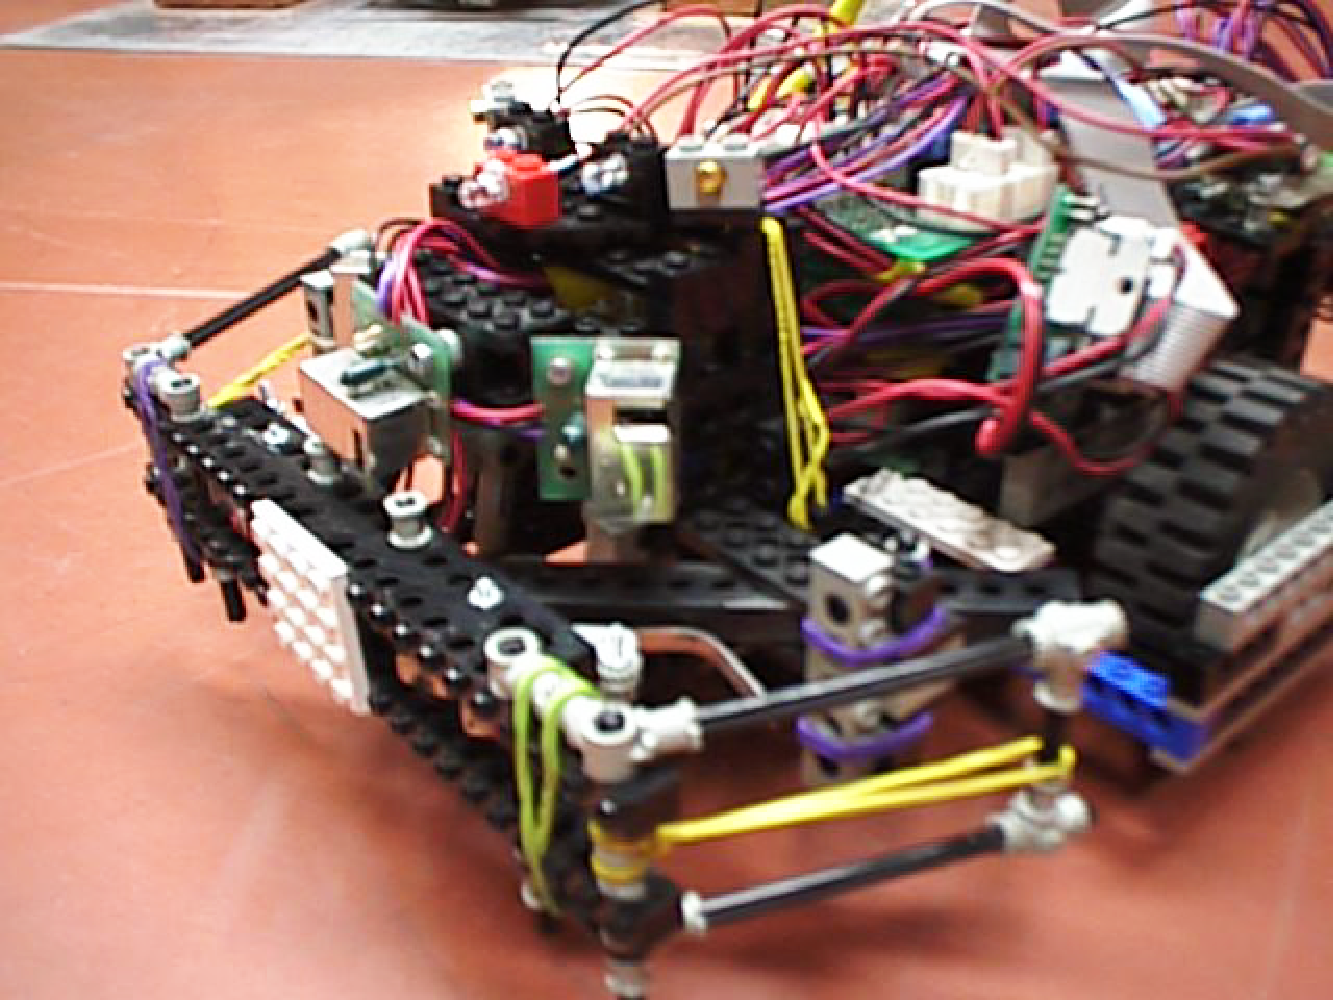
\includegraphics[width=.60\textwidth]{chap1/figs/robot.pdf}}
\caption{Example of a {\it Lego vehicle} built by Tim Smithers based on Lego bricks, a sensori-motor processing board, 
and a variety of 
sensors and actuators. We developed these robots in the early nineties for exploring a behaviour-oriented 
approach to robotics.}
\label{f:plate3}
\end{figure}

Most robots drove around on wheels, but we also used balloons and propellers to build 
flying robots and experimented with a fish-shaped robot which swam in the university swimming pool by wagging 
its tail (see \figref{f:plate4}). 


\begin{figure}[htbp]
  \centerline{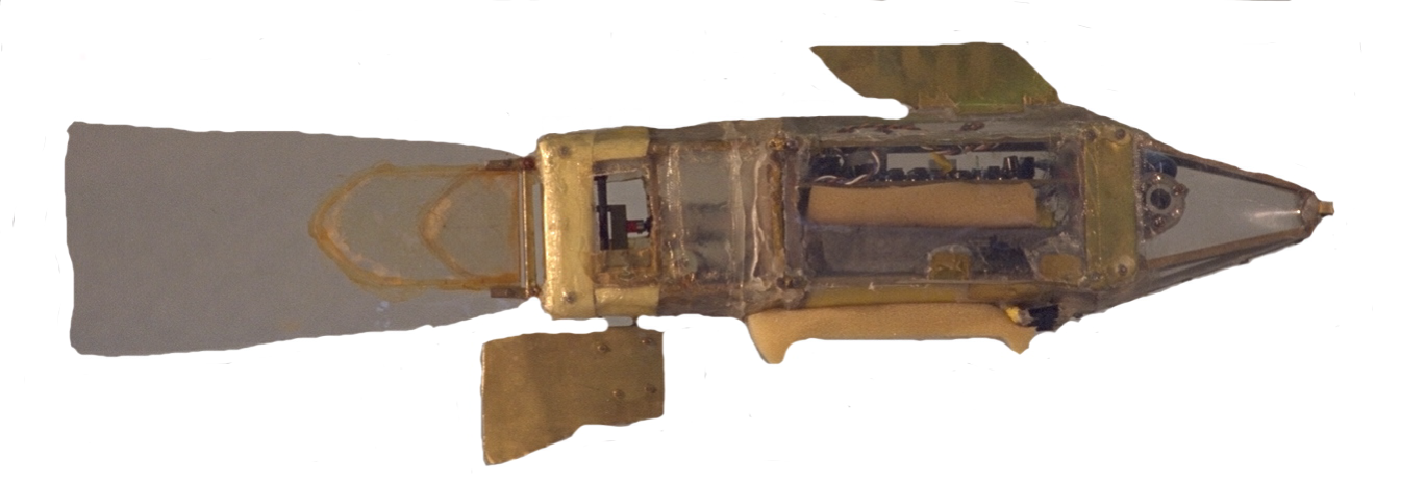
\includegraphics[width=.85\textwidth]{chap1/figs/fish.pdf}}
\caption{``Artificial fish'' built by Miles Pebody to explore influence of robot bodies on behaviour. The fish could swim around by wagging 
its tail and avoid obstacles based on infrared sensing.}
\label{f:plate4}
\end{figure}

To investigate the role of the environment in shaping the
evolving sensori-motor capacities of these robots, 
we built various robotic 
ecosystems in which robots could recharge themselves but also
had to work for their living by 
dimming lights that took away energy from the total energy 
flowing in their ecosystem (see \figref{f:plate6}). Visitors
to our lab could see robots helping each other or 
engaging in fierce competition for
the resources available for survival. In all of this
research, we tried to see how far behaviours would
autonomously evolve, in other words we tried to find 
mechanisms by which the robots would bootstrap themselves 
towards greater sensori-motor complexity. One of the 
main lessons from these experiments was that 
explanations for cognition lie partly outside the brain 
of the individual agent: The environment, the body, the 
sensori-motor apparatus and the behaviour of the other 
agents all partly shaped their capacities and 
further development.\footnote{This approach is also known as {\it situated cognition}. 
\cite{Clancey:1997}, see also: \cite{Varela:1991}.}


\begin{figure}[htbp]
  \centerline{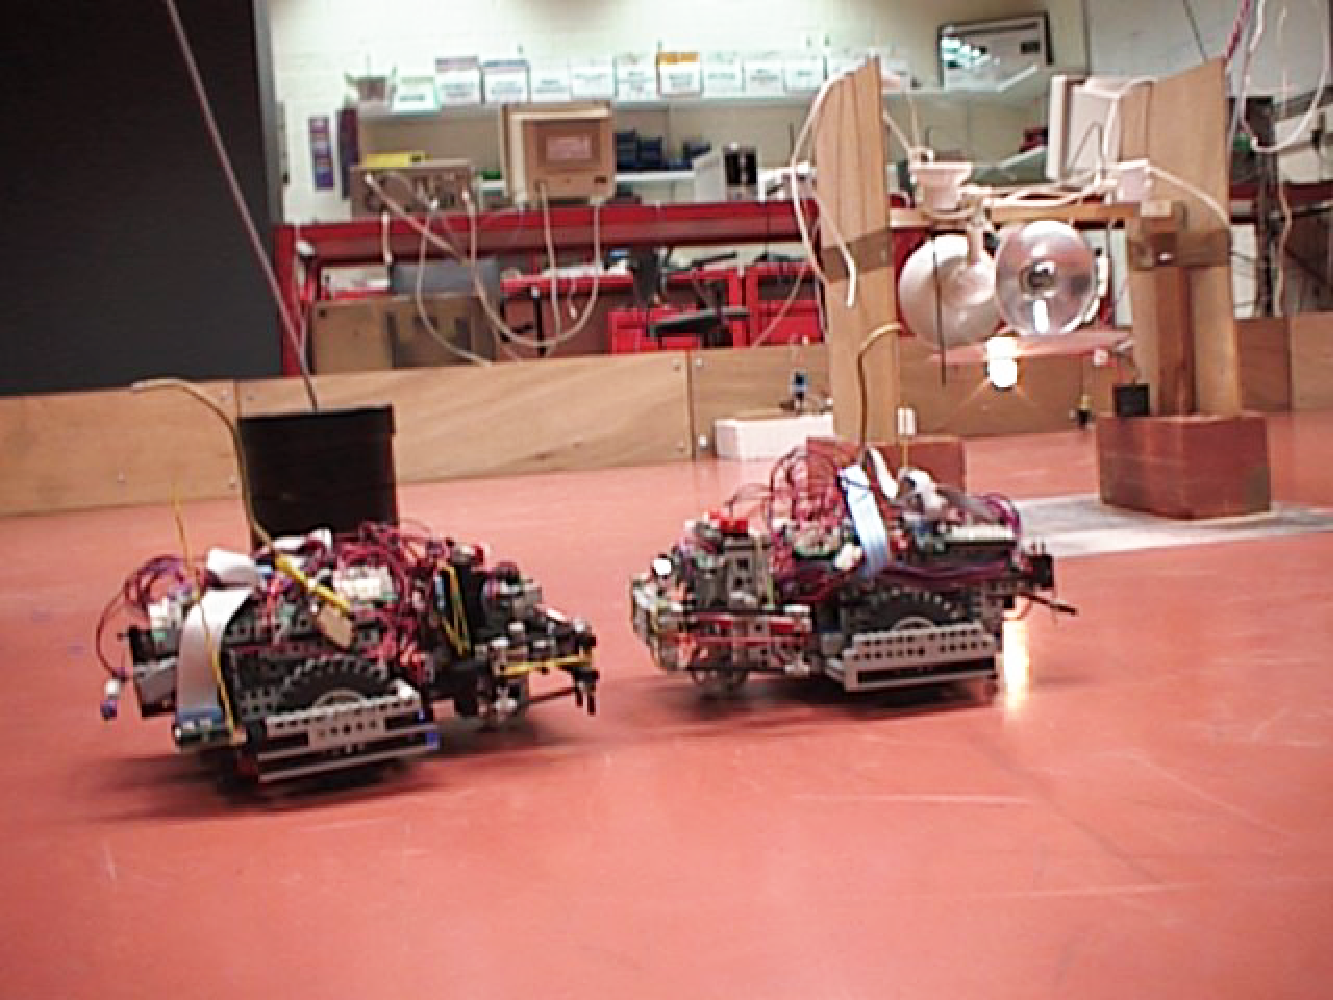
\includegraphics[width=.80\textwidth]{chap1/figs/ecosystem.pdf}}
\caption{This ecosystem was designed together with David McFarland (Oxford University) to explore 
emergent cooperation and competition. The robots in the form of lego vehicles could recharge themselves in the charging 
station (shown in the right top corner). But they had to ensure that there was enough energy in the charging 
station by dimming a light in black cylinders by pushing against them.}
\label{f:plate6}
\end{figure}

Many fascinating tales can be told about this research but the intelligence being exhibited 
by these autonomous robots hardly seemed worthy of the name. Yes, they learned
by themselves how to avoid obstacles, how to recharge themselves
in a charging station, or how to co-ordinate efforts 
to exploit the resources in the ecosystems we had built for 
them. But critical observers did not see much more than 
rat intelligence and they were right. The original 
goal of reaching human 
cognitive levels, as observable for instance in 
expert problem solving or conversations in natural
language, remained elusive. The 
traditional artificial intelligence
approach of explicitly programming symbolic intelligence
still gave far superior performance in tasks requiring
cognition. Clearly, essential theoretical concepts were 
missing for a truly bottom-up approach to succeed. 

In the summer of 1995, a clear breakthrough occurred.  
I was working as a visiting researcher in the Sony
Computer Science Laboratory in Tokyo, invited by its director
Mario Tokoro. Reflecting on our 
experiments from a distance, two new ideas occurred to me. 
First of all, language may have been the missing key
in the initial experiments. Language may 
be a necessary route by which the human cognitive system
bootstraps itself autonomously, in tight interaction with the
environment and aided by a community of other
language speakers. This suggested that if we wanted
to have emergent
forms of cognitive intelligence, we needed to go the same 
route. Second, the principles and mechanisms that had been
pouring out of the study of complexity had to be
relevant to understanding the origins and evolution of language,
because they provided generic explanations for how complexity 
may emerge. These principles include 
self-organisation, structural coupling, 
selectionism, level formation, 
and many others (\citealt{Nicolis:1989}). The field of {\it artificial life} brings together researchers
exploring the insights of complex systems with computational
and robotic experiments (see: \citealt{Langton:1995}).

Together with 
other researchers interested in the then-arising field of `artificial life', I had 
already been simulating path formation in 
ant societies and other biological phenomena exhibiting 
an emergence of complexity. It dawned on me that the
importance of these mechanisms for bootstrapping intelligence and
language might be much greater than 
thought so far.\footnote{The following reference provides a general survey of similar work in 
the area of lexicon formation: \cite{Steels:97b}. 
A representative sample of work on syntax is \cite{Briscoe:1999}.}

\clearpage
Back in Brussels, an extremely exciting but very 
intense period of research started as I tried to 
apply these principles to language
and subject them to experimental 
scrutiny.\footnote{The earliest papers on these mechanisms are in: \cite{Steels:95b} and 
\cite{Steels:96a}.}
We very quickly built a first 
prototype of a {\it Talking Head} with our own hardware
and low-level software (see \figref{f:plate7}) 
and experimented with language games on mobile 
robotic agents.\footnote{The electronics and tracking software for this 
active camera were built by Tony Belpaeme. The mobile
robot experiments were conducted with Paul Vogt. 
Other early work on the grounding and autonomous acquisition of 
language-like communication systems by robotic systems is 
described in \cite{Steels:97g}. See also: \cite{Billard:1998}.}
New fundamental insights and discoveries emerged almost daily. 
The first experiments, particularly in grounding
language on real robots, were extremely difficult but we 
were clearly making steady progress. 


\begin{figure}[htbp]
  \centerline{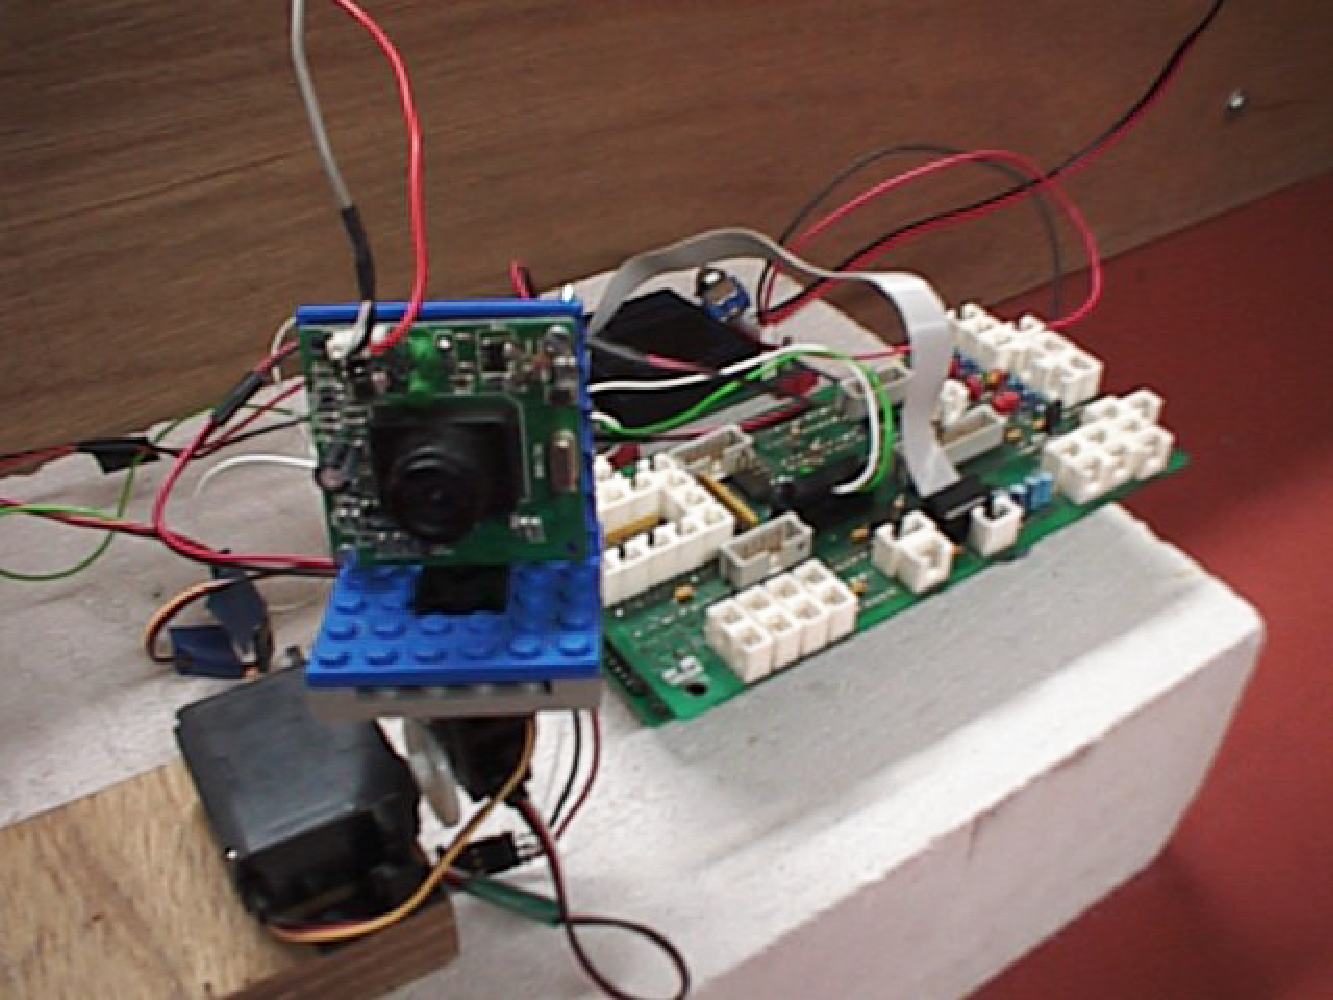
\includegraphics[width=.70\textwidth]{chap1/figs/eye.pdf}}
\caption{First prototype of a {\it Talking Head} camera with 
associated electronics built by Tony Belpaeme. The camera is capable to track moving images. }
\label{f:plate7}
\end{figure}

As my research programme grew more radical, it became more 
and more difficult to get funding. 
European research and development programmes were 
increasingly demanding short-term projects that targeted information
technology products already available on the American or Japanese 
market. Increasingly, my
research proposals were being rejected and running projects were
cut off,
as reviewers could not see direct short-term 
commercial benefits. All this was endangering the further existence
of my Brussels laboratory, whereas I, paradoxically, thought that
our research had never been more promising. 
Fortunately at this critical moment Mario Tokoro
helped me again in a crucial way. He understood what I was
hoping to achieve and ensured secure and stable resources from 
the Sony Corporation. At the end of 1996, I consequently set up a new research
structure in Paris, a spin-off from the Sony Computer Science
Laboratory in Tokyo, where the bulk of the research reported
in this book could be done in almost ideal circumstances. 
The Paris research was complemented with many important 
contributions from my graduate students
at the VUB AI Laboratory in Brussels. 

\section{Beyond Turing}

A scientific experiment creates, in a controlled
and repeatable way, phenomena which shed light on
similar phenomena observed in the natural
world. Initially there is
always some discussion about the relation between 
the artificially created phenomena and the natural
phenomena. Galileo dropped cannon balls from
the tower of Pisa and claimed that these experiments validated 
a general theory of falling bodies; but his contemporaries 
objected that birds graceously landing on a roof can
also be seen as falling bodies, so how general was 
his theory really?  

When dealing with cognitive phenomena such as language
and meaning, the same problem arises. To what extent
do the languages constructed by the Talking Heads count
as languages? Does it make any sense to say that these robotic 
agents categorise their world? Do the Talking
Heads learn? Do they genuinely understand each other? Do they 
understand us? To what extent 
is there a real increase in syntactic 
complexity? Intense discussions about whether cognitive phenomena can 
be recreated in artificial systems 
have raged since researchers have been exploring this 
route, and they have been shown extremely difficult to resolve to 
everyone's satisfaction. 

It seems unavoidable that there is disagreement because 
judgements about cognitive capabilities are to some 
extent subjective. Most people ascribe more intelligence
to their pets than a casual observer is willing to admit. 
In any case, judgements should clearly rest with humans, and
definitely {\itshape not} with the designers 
who are all too keen to call their systems intelligent. 
This was clearly recognised by Turing \is{Turing test} when he devised
his famous Turing test.\footnote{The Turing test is originally described in 
\cite{Turing:1950}.} Turing started from a popular societal 
game of his time, where an observer had to tell through
a dialog whether he was talking to a man or a woman. 
He proposed to call a computer program intelligent when 
it was capable of playing the role of a man or woman
so well that the observer could no longer tell whether
a person or a computer program was playing the game. 
The Turing test has rightfully been criticised as being
on the one hand too difficult, because it is completely 
open-ended, and on the other hand too narrow, because it 
does not incorporate important aspects of intelligence such 
as learning or sensori-motor intelligence. The only way 
to have a decent showing in the Turing test is to
cheat, i.\,e. to let the computer mimic intelligence 
by manipulating symbolic patterns without any notion of what 
they mean. It is therefore desirable to have an alternative
set up which still preserves some of Turing's original 
ideas. 

The goal of the Talking Heads experiment is not to demonstrate 
an artificial intelligence with the same capacities as 
human intelligence, but to perform
scientific experiments so as to examinine aspects 
of a theory of the origins of language and meaning. 
However, as in Turing's proposal, the public should be 
the ultimate judge whether cognitive phenomena are taking
place, and the artificial agents should be able to play their role
in interaction with humans. 
Sound scientific methodology requires that 
the experimental apparatus is a white box which can be fully probed 
by anyone who wants, that the experiments are repeatable, 
and that the phenomena that are generated 
(for example, the complexity of the lexicons or 
grammars) can be 
compared by anyone to human cognitive phenomena in order to gage 
their similarity and thus their relevance for understanding
human cognition. 

In 1999, a golden opportunity presented itself to 
expose our theories and systems to public scrutiny and thus solicit
judgements from a wide range of human observers. Barbara
Vanderlinden and Hans-Ulrich Obrist, two internationally 
renowned young curators, had been put in charge of 
an important art event in the city of Antwerp (Belgium)
and made the brilliant decision to organise a 
confrontation/co-operation between art and 
science.\footnote{The catalogue of this event (\citealt{Obrist:1999}) gives an idea of 
the other laboratories and the coming together of art and science.}
They invited \is{Laboratorium exhibition}
artists and scientists to set up 
a public laboratory in the city and conduct experiments 
from the viewpoint of their discipline. This is how 
the Talking Heads experiment came to be installed in 
a public space in Antwerp and how thousands of people, 
some more bewildered than others, took part in the first
ever large-scale public experiment in artificial intelligence. 
Everybody was encouraged to interact with the robots and 
to try and understand what was going on. This was not an obvious
thing to do because the Talking Heads
construct their own language and their own conceptualisation of 
the world. Understanding what they are talking about resembles the work 
of an anthropologist who is studying the language and
conceptualisations of a newly discovered tribe living
secluded in the rainforest. 

The {\it Laboratory for cognitive robots and 
teleportation} that housed the 
Talking Heads experiment also contained  
a documentation room in which the audience could 
get additional background information and 
provide feedback and commentary 
on the experiment. We created a website that was accessible 
worldwide through the Internet. This allowed viewers from anywhere
in the world to follow the dialogs, inspect the lexicons
and ontologies (sets of perceptually grounded concepts) 
of the robots, and even interact remotely with the 
physical robots, playing language games 
and doing their own experiments. We also added
other physical sites in Tokyo, Brussels, Paris, Amsterdam, 
San Jose (US) and other places, to increase the environmental complexity that 
the agents could experience. 

\enlargethispage{1\baselineskip}
The massive response and thoughtful judgements of the 
public were crucial to validate many aspects of the 
theories put forward in this book. 
But the interactions with a broad public and
the intense discussions that it generated also added new
dimensions to the research. First of all, a whole 
new type of interface between man and machine was
taking shape under our very eyes. In contrast to pre-programmed
computer interfaces, which more often than not make it
difficult to do what one wants, the Talking Heads demonstrated
for the first time the concept of {\itshape negotiated user
interfaces}. The interaction was based on mutual respect
and adaptation of man {\itshape and} machine. Communicative
failure was not fatal but 
an opportunity to fine-tune and negotiate the way communication
would take place in the future. 

Secondly, the Talking Heads experiment turned out to be 
an ideal learning environment for raising philosophical
issues. Children and adults alike
started to ask questions about the nature of
meaning, the relation between language
and reality, the mind-body problem, 
the origins and evolution of language, 
consciousness, social identity, and so on. They 
start to play language games among themselves and some of
them reported profound changes in the way they 
think about language. If these reflections create 
greater tolerance towards other languages and 
the conceptualisations of the world
they implicitly embody, then I consider the
Talking Heads experiment of great societal value, irrespective of
the scientific and engineering breakthroughs
the project has generated. 

\section{The book}

This book describes in detail the rationale behind the 
Talking Heads experiment, the mechanisms that make it
all work, the ontologies and 
languages the agents develop, and what happened
when the Talking Heads were exposed to public scrutiny. 
It studies processes which must already be active in the 
very first stages of language use in the child, and 
must also have been present in the early phases of 
human language genesis. 

The main text contains the
principled line of the argument in a form which is intended to be generally
accessible without compromising exactness. The notes after
each chapter contain references to other work, as well 
as details or additional material of relevance to the 
specialist. Each chapter also contains a set of references to
literature on the same topic. 

This book starts with a preview of the 
experiment and a brief illustration of the core ideas (\chapref{chap:2}). 
I then cover the 
different tasks step-by-step that speakers and hearers must carry out: 
perception (\chapref{chap:3}), conceptualisation (\chapref{chap:4}), 
and lexicalisation (\chapref{chap:5}). Each 
chapter discusses the 
architectural components with which the Talking Heads 
have been endowed and the kinds of cognitive structures that 
the agents generate in interaction with the environment 
and the other agents. \chapref{chap:6} and \chapref{chap:7} then bring all these 
results together and tests the rich complex semiotic dynamics that 
arise when the Talking Heads effectively interact 
with real world environments. 

The research discussed in this book is far from finished. It is 
still science in the making. Many cognitive structures
and capabilities, even very elementary ones arising 
during the first years of human life, are still unveiled. Many
language issues
have not been covered yet. The current set-up 
shows only inklings of what future forms of man-machine
interaction might be like. Nevertheless, I believe that 
the hypotheses proposed in this book, and the 
methodology of experimentation that has been used to 
explore these hypotheses, open new venues for 
a scientific understanding of the human mind. Building 
artificial systems that exhibit cognitive capabilities
does not de-humanise the mind, in the 
same way as the telescope does not demystify the cosmos. 
We see much more and what we see is infinitely more 
beautiful and impressive. 

%\end{document}
